\documentclass[10pt,tikz,border=1mm]{standalone} 
\usepackage{mathpazo}
\usepackage[T1]{fontenc}
\usetikzlibrary{arrows.meta}
\tikzstyle{dot}=[circle,fill=black,inner sep=1pt]
\tikzstyle{arrow}=[-{Stealth[scale=2]},thin,text=black]
\begin{document}
	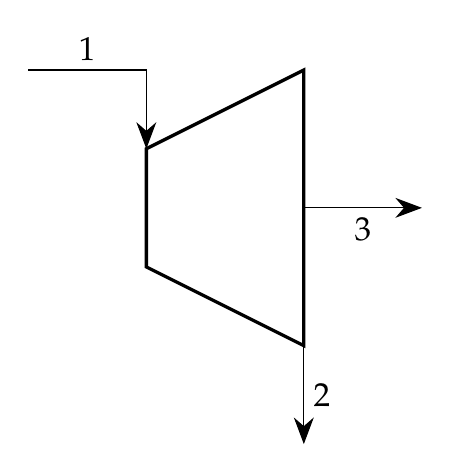
\begin{tikzpicture}[font=\large]
		%\draw[step=1cm,black!20,very thin] (0,0) grid (6,6);
		\coordinate (A) at (2,3.25);
		\coordinate (B) at (2,4.75);
		\coordinate (C) at (4,5.75);
		\coordinate (D) at (4,2.25);
		\coordinate (E) at (4,4);
		\coordinate (B1) at (2,5.75);
		\coordinate (B2) at (0.5,5.75);
		\coordinate (E1) at (5.5,4);
		\coordinate (D1) at (4,1);
		\draw[very thick] (A)--(B)--(C)--(D)--cycle;
		\draw[arrow] (B2) -| (B);
		\path (B2) -- node[above]{1} (B1);
		\draw[arrow] (D) -- node[right]{2} (D1);
		\draw[arrow] (E) -- node[below]{3} (E1);
	\end{tikzpicture}
\end{document}